
\chapter{Experimental Evaluation}

In this section we discuss our experimental evaluation.
First we describe the benchmarks with datasets used in the experiments.
Afterwards, we discuss our results concerning the instrumentations for profiling our work metric.
Finally we present the results of the online {\itercomp}.

We implemented the instrumentations in LLVM 4.0.
The target platform is a Linux-4.4.27 system with an Intel Core i7-4770 3.40GHz Skylake~CPU with 16~GiB RAM.

\section{Benchmarks}

%{\Itercomp} is essentially based on repeatedly trying out a large number of compiler optimisations until the best combination of compiler optimisations is found for a particular program.
%Our main goal is to speed up {\itercomp} while targeting optimal performance across large input datasets.

For the experimental evaluation we have used a subset of the \textit{KDataSets} benchmark suit, which is the same benchmark and dataset suit used by Chen~\etal~\cite{chen10,chen12a}.
The KDataSets contains 1000 different inputs for each one of its benchmark programs.
These benchmarks cover a broad spectrum of application scenarios, ranging from simple embedded signal-processing tasks to common mobile-phone and desktop tasks.
The different inputs try to capture distinct characteristics in terms of workload sizes and how these workloads exercise different control flow paths.
A summary of the benchmark and dataset suit is shown in Table~\ref{tab:kdatasets}.

\begin{table}[h]
\centering
\scalebox{.8}{
\begin{tabular}{|c|c|c|c|}
\hline
\textbf{Program} & \textbf{LOC}    & \textbf{Input file size}            & \textbf{Input description}              \\ \hline % Domain
qsort         & 154    & 32K-1.8M                   & 3D coordinates                 \\ \hline
jpeg\_d       & 13501  & 3.6K-1.5M                  & JPEG images                    \\ \hline
jpeg\_c       & 14014  & 16K-137M                   & PPM images                     \\ \hline
tiff2bw       & 15477  & \multirow{4}{*}{9K-137M}   & \multirow{4}{*}{TIFF images}   \\ \cline{1-2}
tiff2rgba     & 15424  &                            &                                \\ \cline{1-2}
tiffdither    & 15399  &                            &                                \\ \cline{1-2}
tiffmedian    & 15870  &                            &                                \\ \hline
susan\_c      & 1376   & \multirow{3}{*}{12K-46M}   & \multirow{3}{*}{PGM images}    \\ \cline{1-2}
susan\_e      & 1376   &                            &                                \\ \cline{1-2}
susan\_s      & 1376   &                            &                                \\ \hline
adpcm\_c      & 210    & 167K-36M                   & WAVE audios                    \\ \hline
adpcm\_d      & 211    & 21K-8.8M                   & ADPCM audios                   \\ \hline
lame          & 14491  & 167K-36M                   & WAVE audios                    \\ \hline
rsynth        & 4111   & 0.1K-42M                   &  Text files                    \\ \hline
sha           & 197    & 0.6K-35M                   & Files of any format            \\ \hline
\rowcolor{gray!20}
bitcount      & 460    &  -                         & Numbers: random                \\ \hline
\rowcolor{gray!20}
dijkstra      & 163    & 0.06K-4.3M                 & Adjacency matrices             \\ \hline
\rowcolor{gray!20}
patricia      & 290    & 0.6K-1.9M                  & IP and mask pairs              \\ \hline
\rowcolor{gray!20}
mad           & 2358   & 28K-27M                    & MP3 audios                     \\ \hline
\rowcolor{gray!20}
%gsm           & 3806   & 83K-18M                    & Sun/NeXT audios                \\ \hline
ghostscript   & 99869  & 11K-43M                    & Postscript files               \\ \hline
\rowcolor{gray!20}
%ispell        & 6522   & \multirow{3}{*}{0.1K-42M}  & \multirow{3}{*}{Text files}    \\ \cline{1-2}
%rsynth        & 4111   &                            &                                \\ \cline{1-2}
stringsearch  & 338    &  0.1K-42M                 &  Text files                     \\ \hline
\rowcolor{gray!20}
%blowfish\_e   & 863    & 0.6K-35M                   & Files of any format            \\ \hline
%blowfish\_d   & 863    & 0.6K-35M                   & Encrypted files                \\ \hline
%pgp\_e        & 19575  & 0.6K-35M                   & Files of any format            \\ \hline
%pgp\_d        & 19575  & 0.4K-18M                   & Encrypted files                \\ \hline
%rijndael\_e   & 952    & 0.6K-35M                   & Files of any format            \\ \hline
%rijndael\_d   & 952    & 0.7K-35M                   & Encrypted files                \\ \hline
CRC32         & 130    & 0.6K-35M                   & Files of any format            \\ \hline
\rowcolor{gray!20}
bzip2e        & 5125   & 0.7K-57M                   & Files of any format            \\ \hline
\rowcolor{gray!20}
bzip2d        & 5125   & 0.2K-25M                   & Compressed files               \\ \hline
\end{tabular}
}
\caption{Description of the KDataSets with 1000 inputs for each benchmark (Chen~\etal~\cite{chen10,chen12a}).}
\label{tab:kdatasets}
\end{table}

\section{Evaluation of the Instrumentation}

In this section we evaluate the performance of the work instrumentation presented in Chapter~\ref{chap:instr}, comparing between the optimal and the relaxed instrumentation with different thresholds.
%We organise the evaluation of the instrumentation as follows:

\subsection{Static Evaluation}

We first compare static aspects of the instrumentation algorithms.
The naive instrumentation always has 100\% of the basic blocks instrumented, by definition.
Figure~\ref{fig:num-probes} shows percentage of instrumented basic blocks for the optimal and the relaxed instrumentation with different relaxation thresholds.
While Figure~\ref{fig:num-probes} compares the different instrumentation algorithms in respect of the naive instrumentation, Figure~\ref{fig:num-probes-improvement} shows the improvement of the relaxation algorithm over the optimial instrumentation.

\begin{figure}[ht]
    \centering
    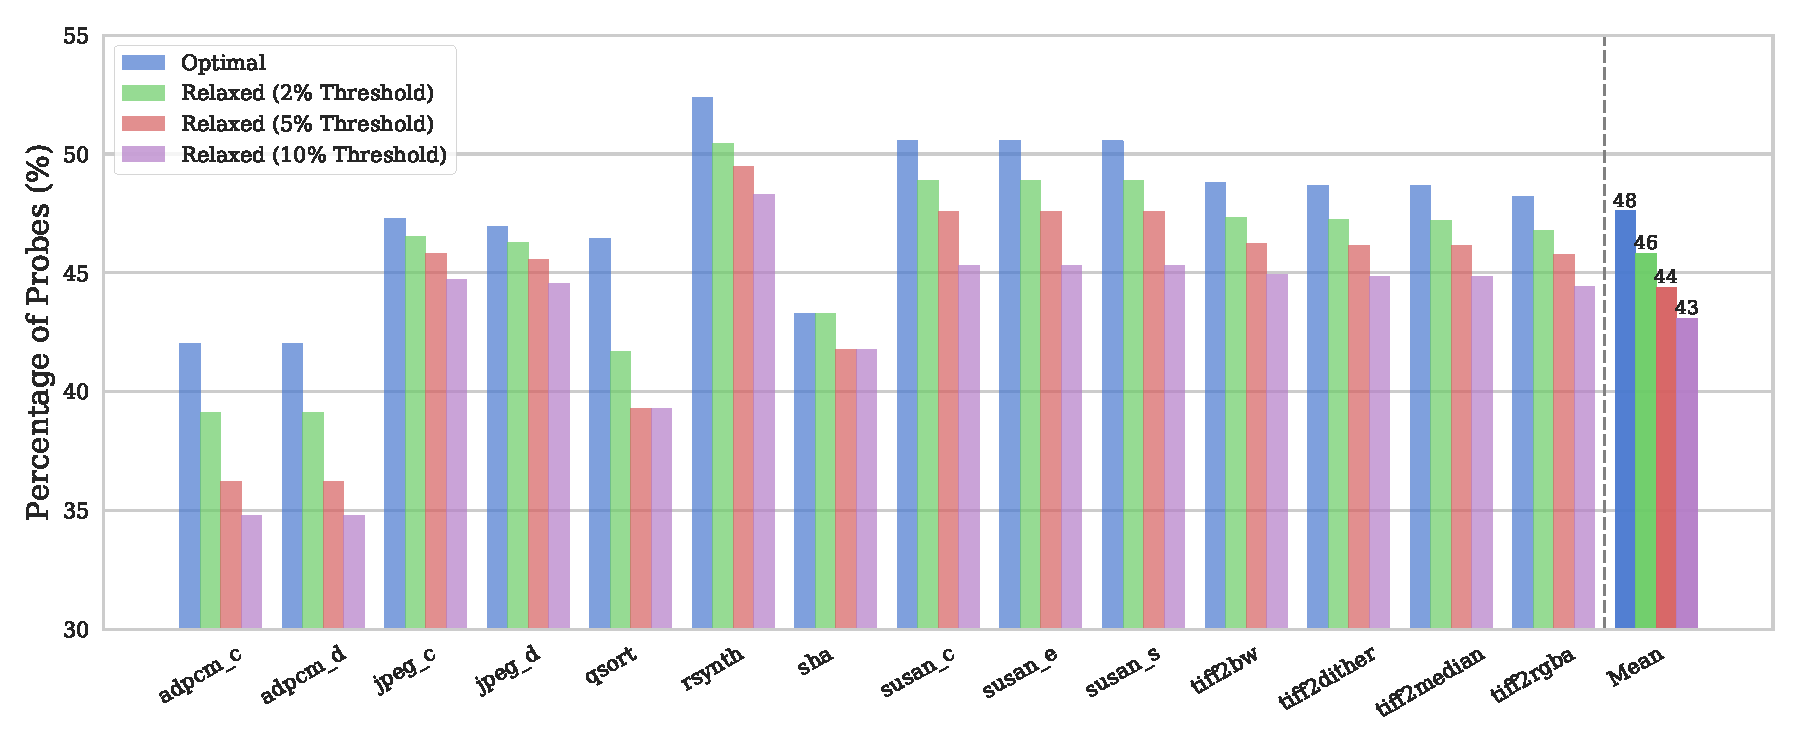
\includegraphics[width=\textwidth]{figs/num-probes.pdf}
    \caption{Percentage of instrumented basic blocks for the optimal and the relaxed instrumentation with different relaxation thresholds.}
    \label{fig:num-probes}
\end{figure}

Even a small threshold of 2\% is able to reduce the number of probes by an average of 5\% compared to the optimal algorithm. 
The \texttt{sha} benchmark was the only benchmark for which a 2\% threshold was not sufficient for further reducing the number of probes.
With a 10\% threshold the relaxation algorithm was able to improve over the optimal instrumentation by an average of 11\%, in terms of the amount of instrumented basic blocks.

\begin{figure}[ht]
    \centering
    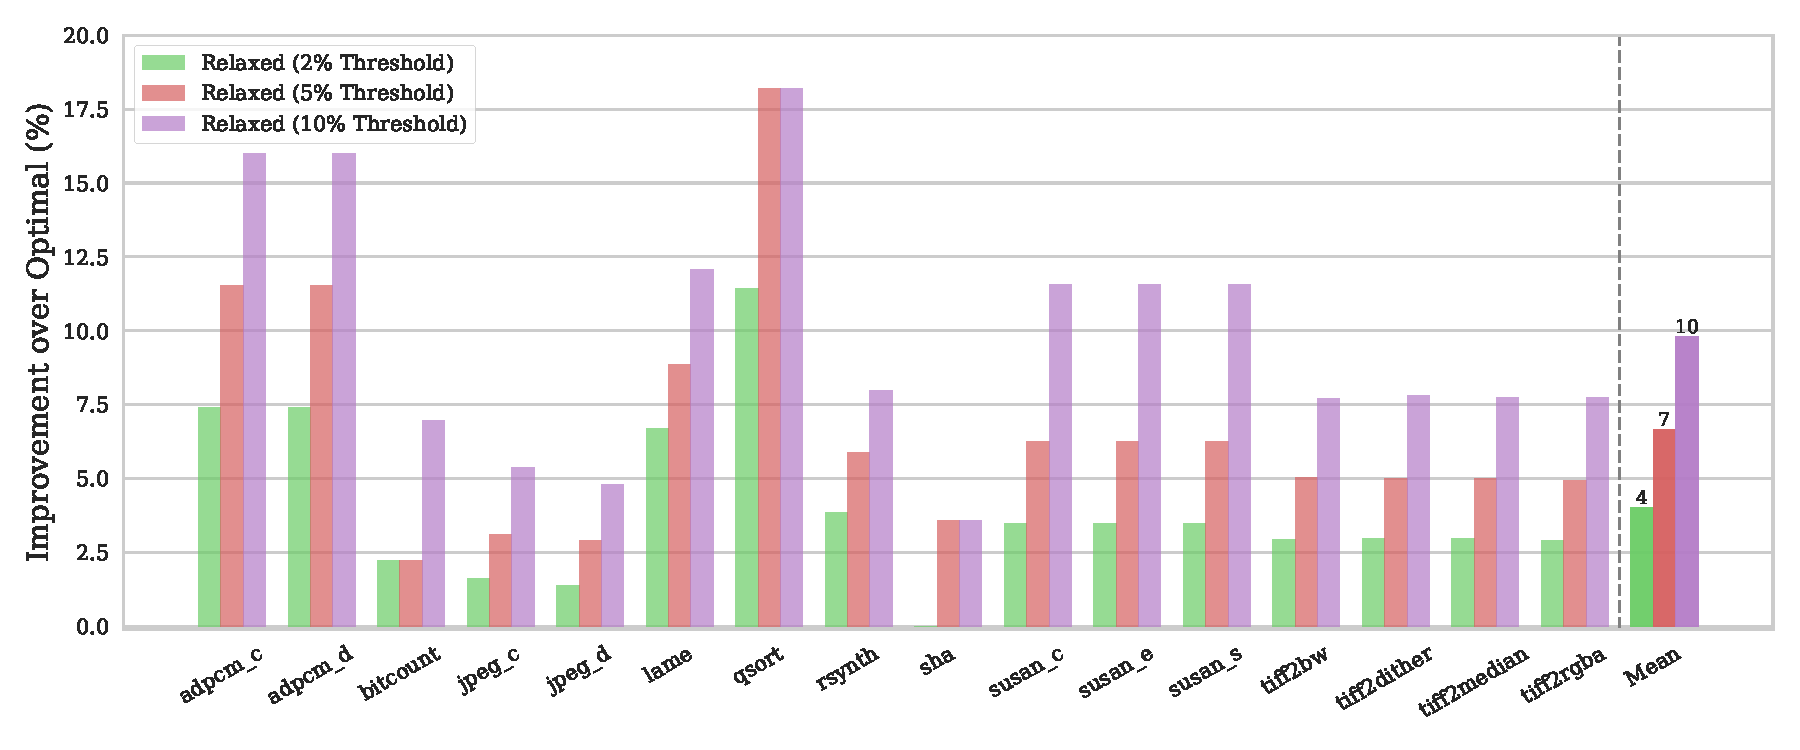
\includegraphics[width=\textwidth]{figs/num-probes-improvement.pdf}
    \caption{Percentage of instrumented basic blocks for the optimal and the relaxed instrumentation with different relaxation thresholds.}
    \label{fig:num-probes-improvement}
\end{figure}

The static errors presented in Figure~\ref{fig:static-instr-error} indicate the amount of error expected by the relaxation algorithm after reducing the number of probes.
This figure shows both the maximum (bars with light colours) and the average (bars with dark colours) static errors observed when relaxing the instrumentation for each DAG of the benchmarks.
Notice that, in most cases, the average static errors are considerably lower than the relaxation threshold, while the maximum static errors are usually close to the threshold.
The average static error shows that in a significant number of DAGs, the relaxation was notably conservative.
This conservatism will be specially evident in the dynamic evaluation.

\begin{figure}[ht]
    \centering
    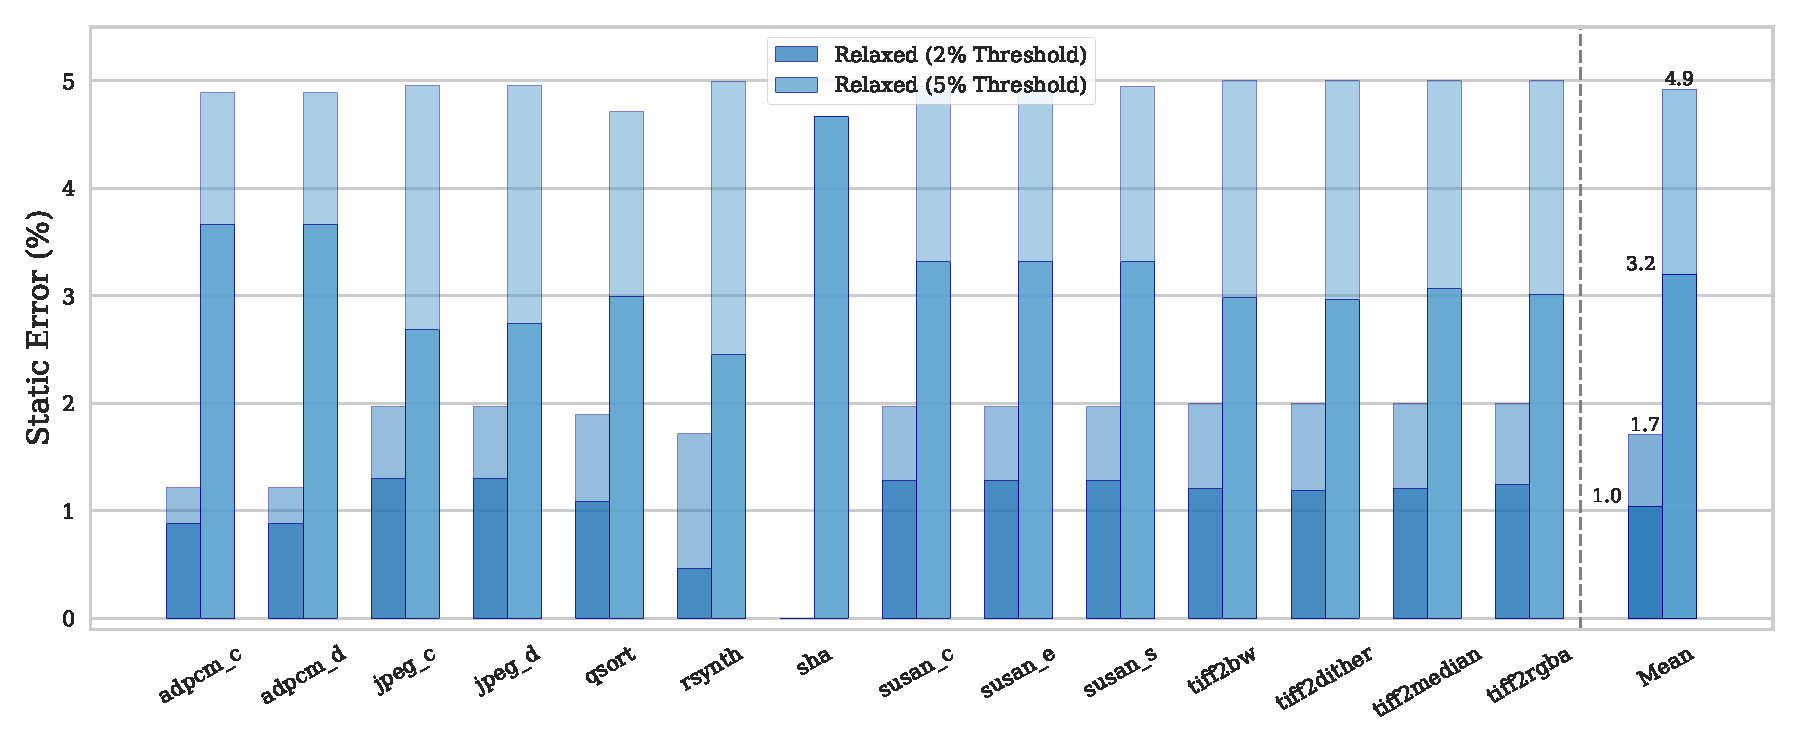
\includegraphics[width=\textwidth]{figs/instr-error.pdf}
    \caption{Average and maximum static error expected for the work profiling, after relaxing the number of probes.}
    \label{fig:static-instr-error}
\end{figure}

\subsection{Dynamic Evaluation}

For the evaluation of the performance overhead that the instrumentation incur to the benchmarks, we measure the wall-clock time of the benchmarks when compiled with thee default \texttt{-O3} optimisation.
For each benchmark, we compute the average overhead over all its 1000 input dataset.
When measuring the wall-clock time for each input, in order to reduce noise, we execute the same input until we have a statistically sound measurement, i.e. we execute until we have an interval no larger than 1\% with 99\% confidence.
Figure~\ref{fig:overhead-O3} shows the performance overhead imposed by the work instrumentation on the benchmarks when compared to their non-instrumented counterparts.
Figure~\ref{fig:overhead-improvement-O3} shows the improvement of the relaxation algorithm over the optimial instrumentation, regarding the reduction in overhead.

\begin{figure}[ht]
    \centering
    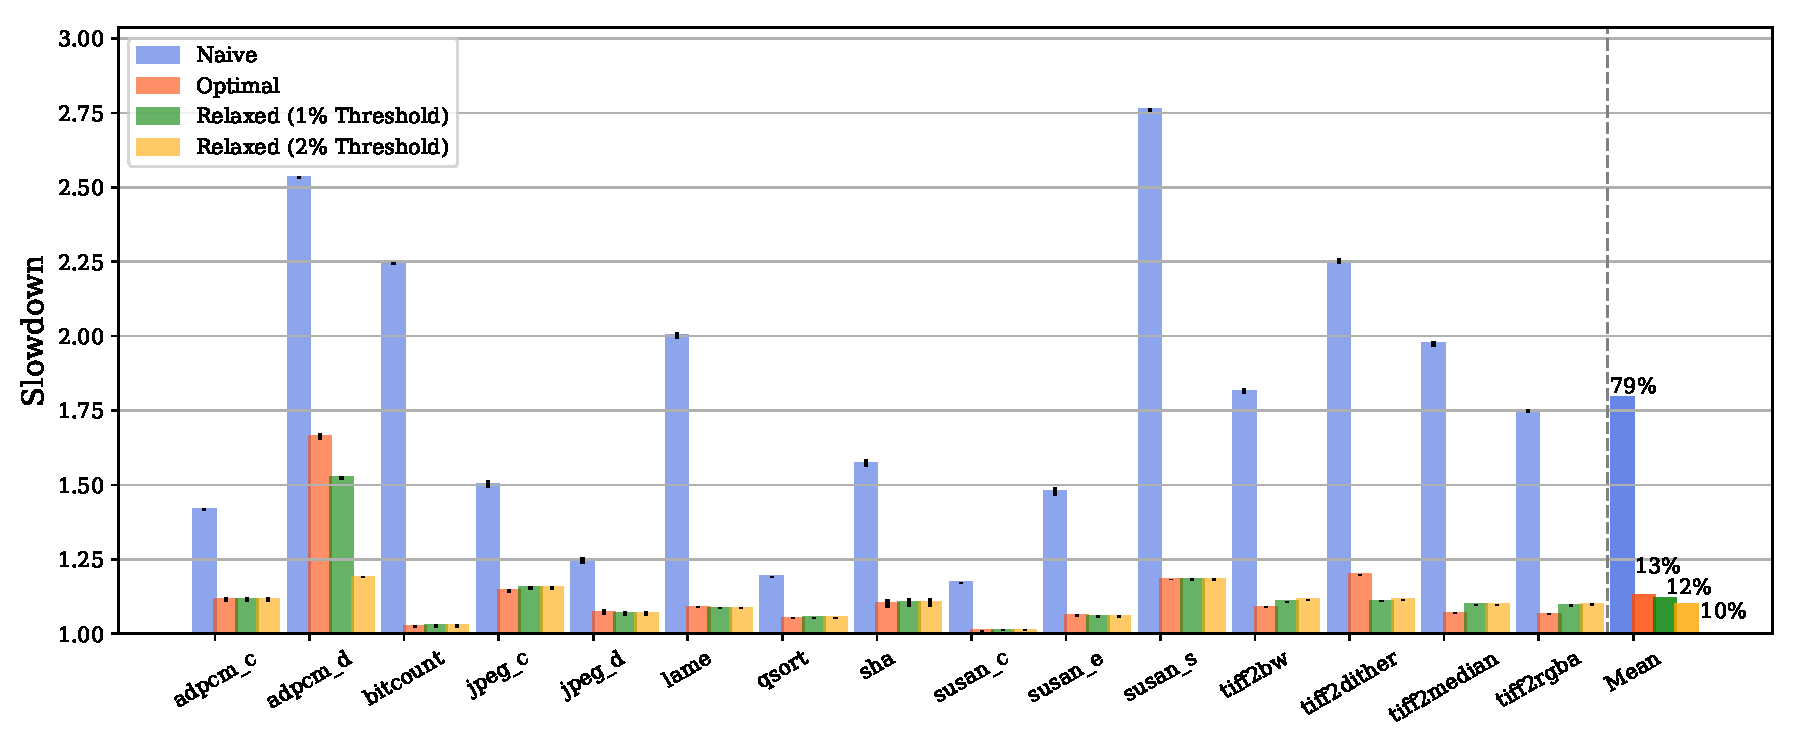
\includegraphics[width=\textwidth]{figs/overhead-O3.pdf}
    \caption{Overhead of the instrumentations compiled with {\texttt{-O3}}.}
    \label{fig:overhead-O3}
\end{figure}

\begin{figure}[ht]
    \centering
    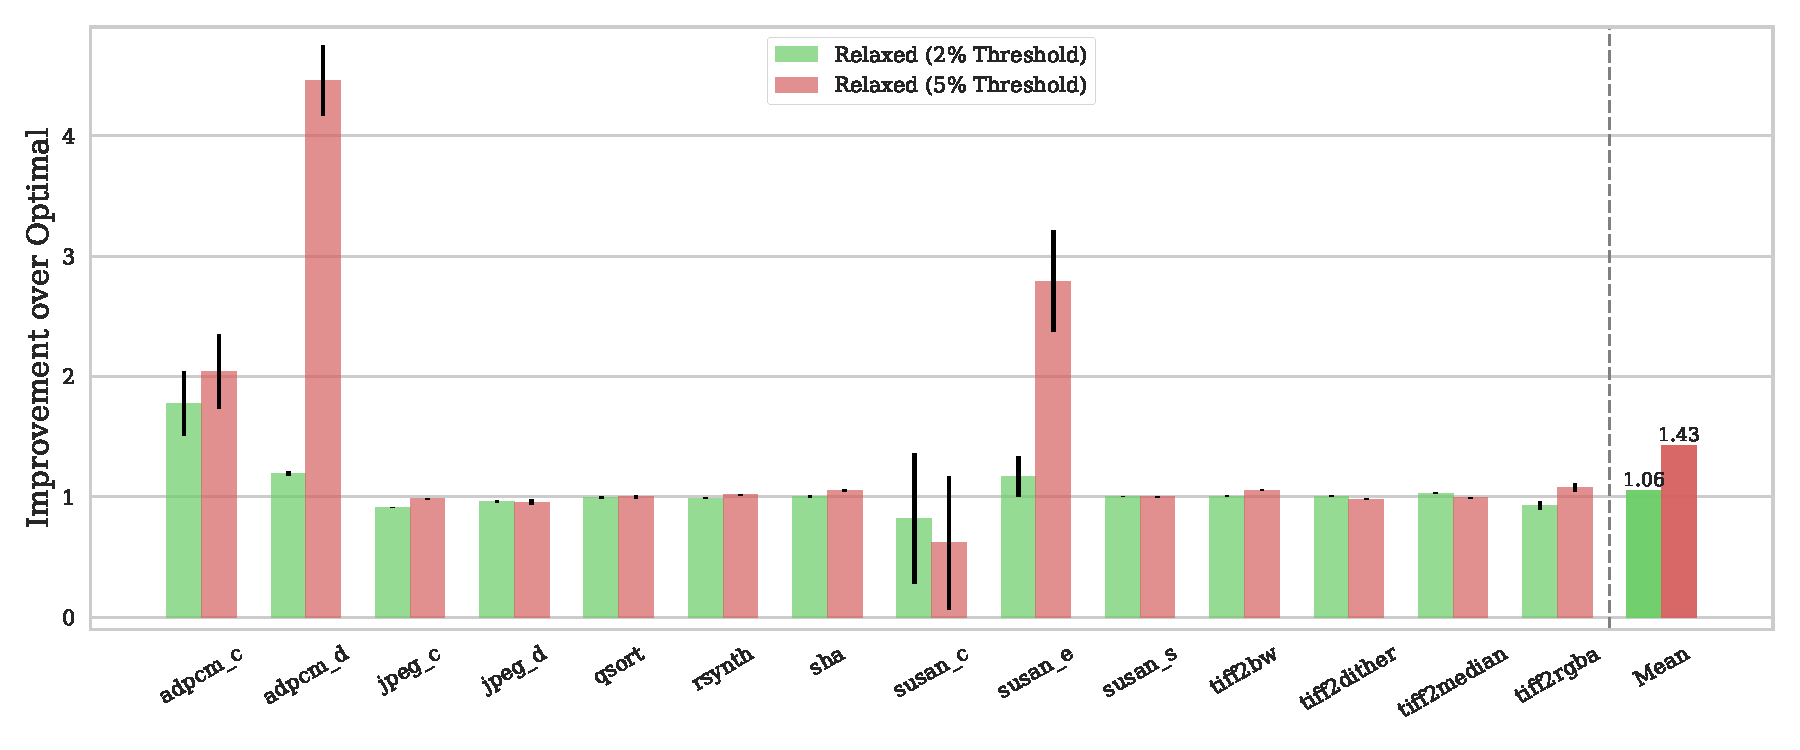
\includegraphics[width=\textwidth]{figs/overhead-improvement-O3.pdf}
    \caption{Overhead of the instrumentations compiled with {\texttt{-O3}}.}
    \label{fig:overhead-improvement-O3}
\end{figure}

Even if we disconsider the exceptional improvement with the \texttt{adpcm\_d} benchmark, the relaxation with a 5\% threshold is able to improve about 20\% on average, over the optimal instrumentation.

\textbf{Profile-guided Instrumentation.}

%\textbf{Code size.}
%\begin{figure}[ht]
%    \centering
%    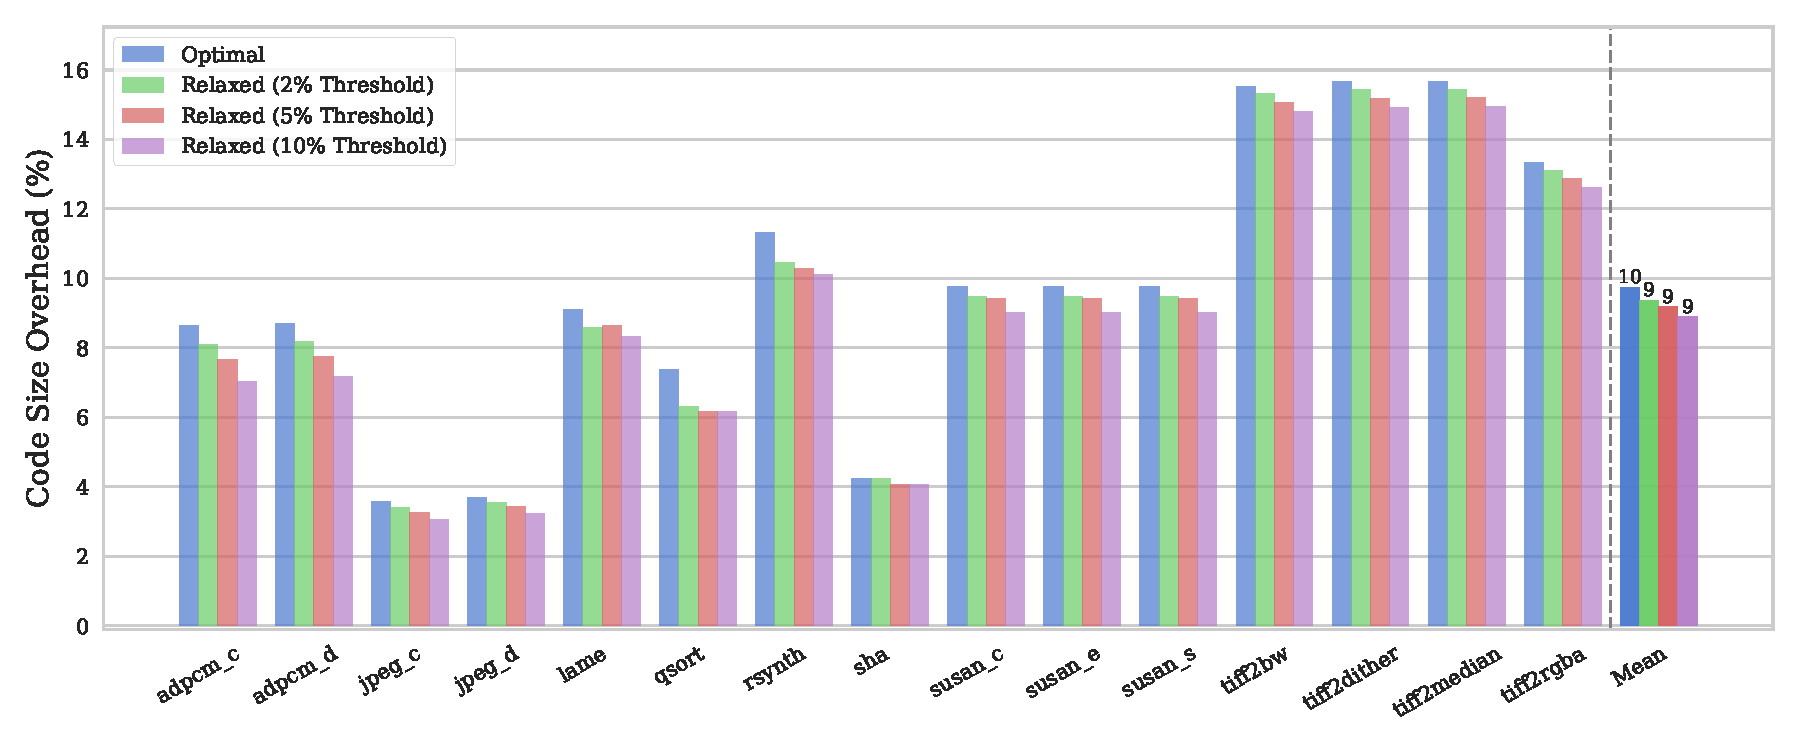
\includegraphics[width=\textwidth]{figs/code-size-probes.pdf}
%    \caption{Percentage of instrumented basic blocks for the optimal and the relaxed instrumentation with different relaxation thresholds.}
%    \label{fig:num-probes}
%\end{figure}
%
%\begin{figure}[ht]
%    \centering
%    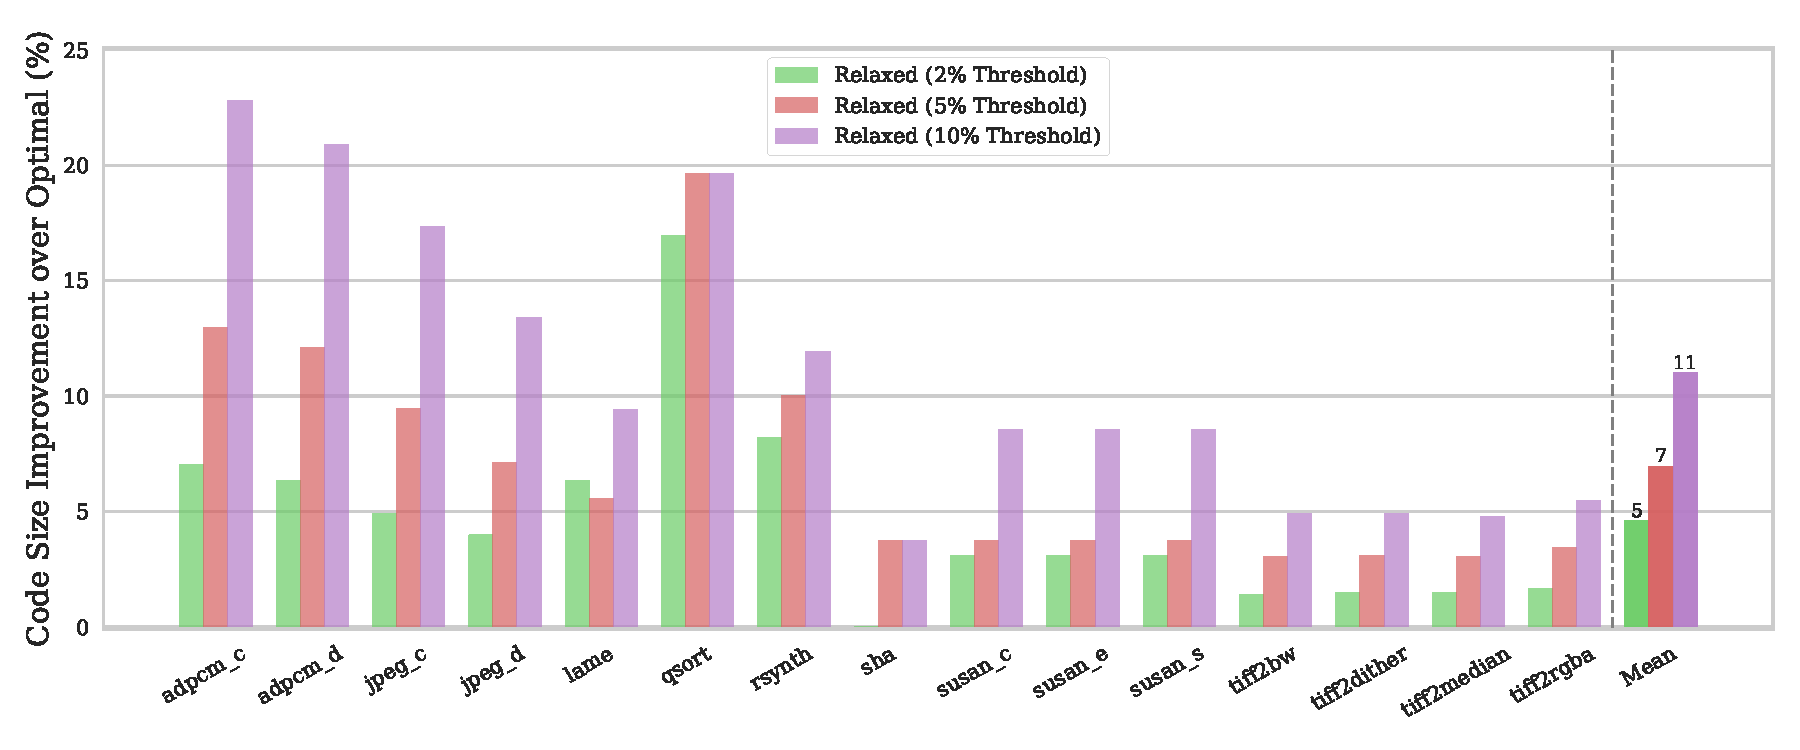
\includegraphics[width=\textwidth]{figs/code-size-probes-improvement.pdf}
%    \caption{Percentage of instrumented basic blocks for the optimal and the relaxed instrumentation with different relaxation thresholds.}
%    \label{fig:num-probes-improvement}
%\end{figure}


%In this section we discuss the three baseline implementations that will be used for assessing the quality of the proposed metric.

%\vspace{1ex}
%\noindent \textbf{{\Itercomp} over a single input}

%Most of the existing {\itercomp} studies find the best optimisation though repeated runs on the same input.
%Although this approach will usually lead to sub-optimal performance across large input datasets, it provides a good baseline when considering the complexity and resonably low compile-time regarding iterative optimising compilers.
%If $M$ is the total number of combinations of compiler optimisations, this approach requires $O(M)$ runs of the program being optimised.
%We can consider two main scenarios:
%\textit{($i$ - best case scenario)} after selecting the optimisation over each individual input, consider the one with best performance across the whole input dataset;
%\textit{($ii$ - expected scenario)} after selecting the optimisation over each individual input, consider the average case of their performance across the whole input dataset.

%\vspace{1ex}
%\noindent \textbf{{\Itercomp} across large input datasets}

%Recent work on {\itercomp} have been targeting optimisation across multiple inputs~\cite{fursin07,chen10,chen12a}.
%If $N$ is the number of input test cases and $M$ is the total number of combinations of compiler optimisations, they perform a total of $O(NM)$ runs of the program being optimised.
%Similarly to what have been discussed previously, there are different ways for how to determine the optimal combination of compiler optimisations across multiple inputs.
%It is possible to tune the selection of the program-optimal combination to minimise risk or to maximise average performance.
%A compromise-based selection criterion could be to maximise average speedup with minimised variance.

\subsection{Case Studies}

\noindent \textbf{Analysis of the Best Improvement in Overhead: \texttt{adpcm\_d}}

The \texttt{adpcm\_d} benchmark is the most critical case amongst the evaluated benchmarks, with an overhead of about 59\% for the optimal instrumentation.
This benchmark consists mainly of a single hot loop with several branches inside it, as depicted by Figure~\ref{fig:adpcm_d-cfg-instr}.
The relaxation algorithm is able to reduce this overhead down to about 47\% (with a static error threshold of 2\%) and 14\% (with a static error threshold of 5\%) by removing only one and two probes from the hot loop, respectively.
These overhead reductions represent a 20\% and 4.5$\times$ improvement over the optimal algorithm, with 2\% and 5\% relaxation threshold respectively.
The two relaxed probes were placed in branches, inside the hot loop, with a high probability of being taken, but with a small contribution to the total amount of work measured in the loop.

\begin{figure*}[htb]
    \centering
    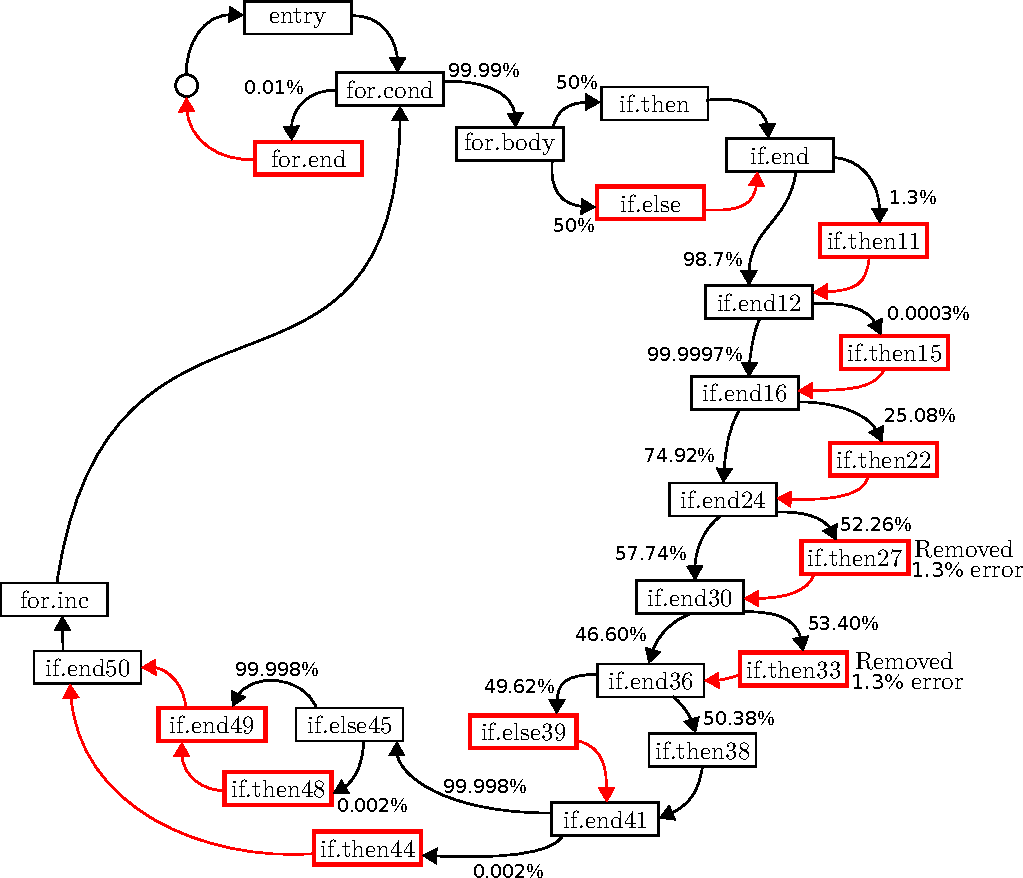
\includegraphics[width=0.8\textwidth]{figs/adpcm_d-cfg-instr.pdf}
    \caption{CFG of the function that contains the hot loop of the \texttt{adpcm\_d} benchmark.}
    \label{fig:adpcm_d-cfg-instr}
\end{figure*}

Figure~\ref{fig:adpcm_d-probes-err-freq} shows all the probes necessary for the function that contains the hot loop of the \texttt{adpcm\_d} benchmark.
Notice that the relaxation was able to remove all probes with an static error lower than the 5\% threshold.
Because these probes were placed in basic blocks with a considerable execution frequency, their removal resulted in a significant reduction in performance overhead.

\begin{figure*}[htb]
    \centering
    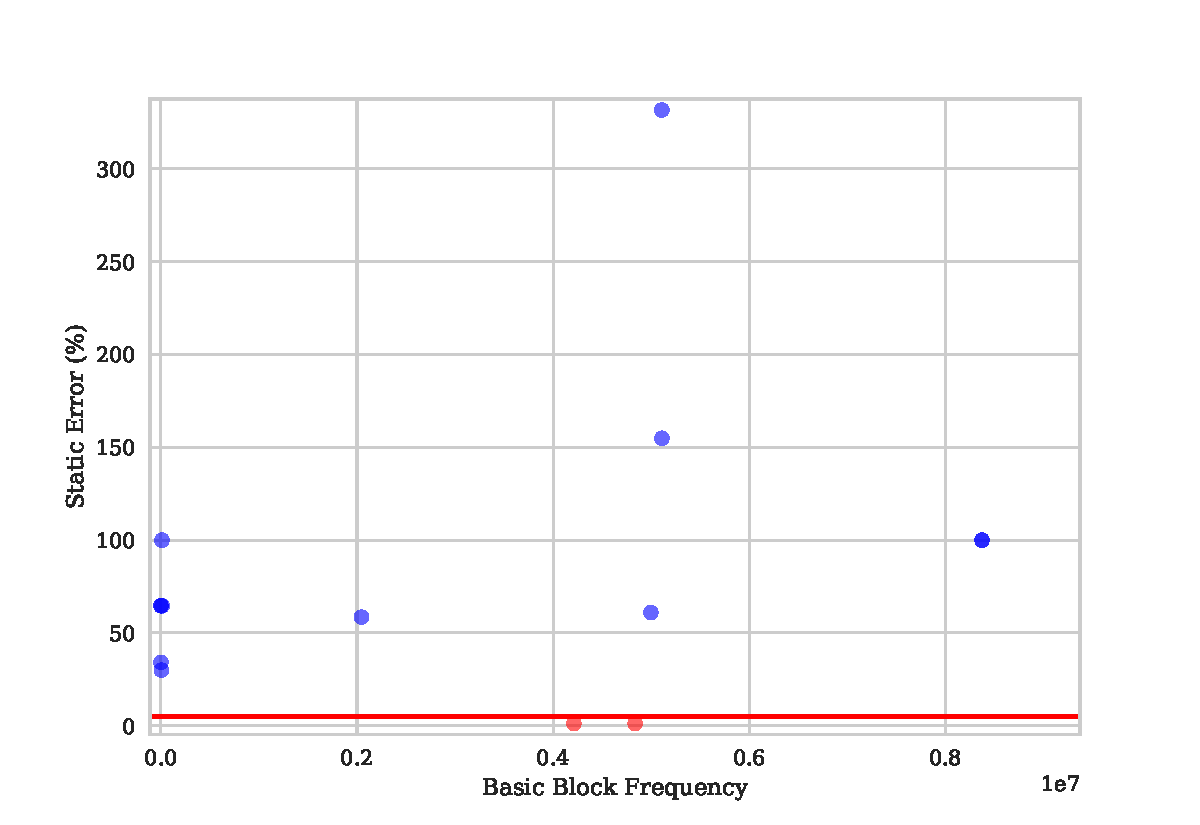
\includegraphics[width=0.8\textwidth]{figs/adpcm_d.pdf}
    \caption{Comparison between probe frequency and static error for the \texttt{adpcm\_d} benchmark. The red line marks the 5\% threshold limit.}
    \label{fig:adpcm_d-probes-err-freq}
\end{figure*}


\noindent \textbf{Analysis of the Abnormal Regression: \texttt{susan\_c}}

\begin{figure*}[htb]
    \centering
    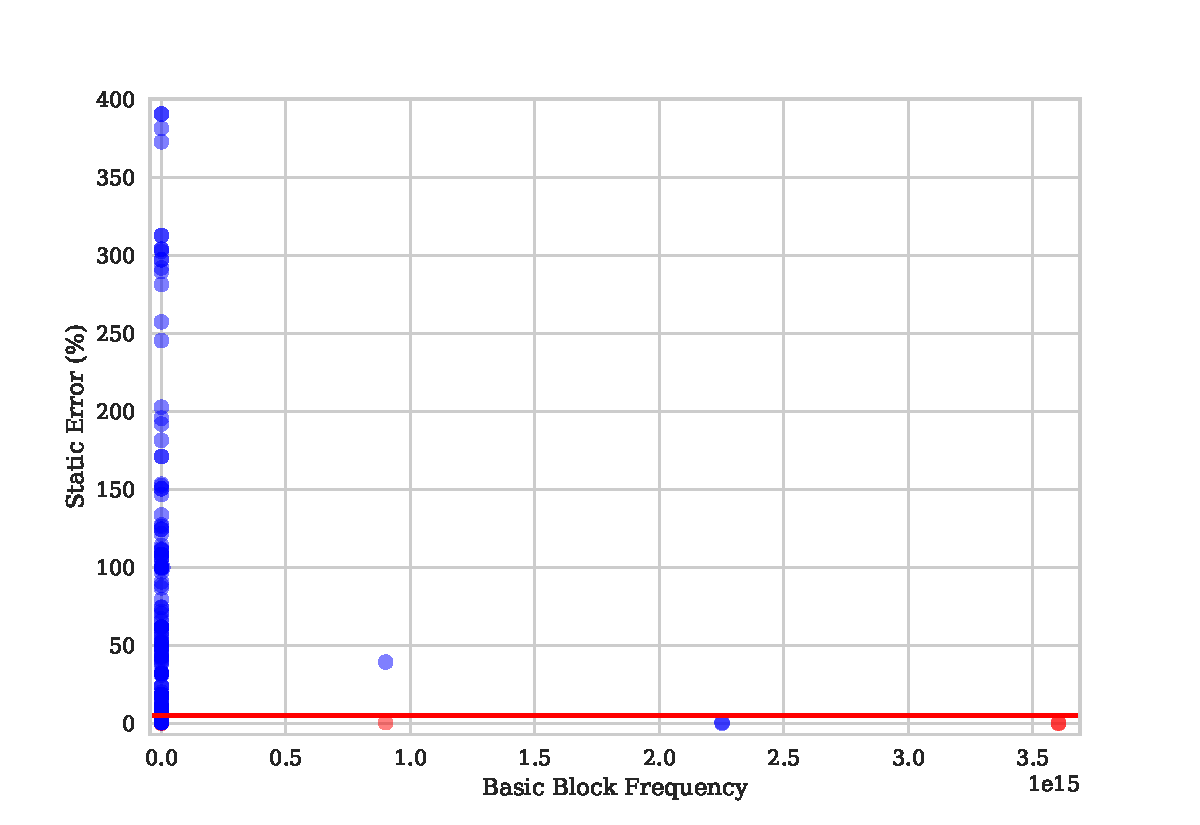
\includegraphics[width=0.8\textwidth]{figs/susan_c.pdf}
    \caption{Comparison between probe frequency and static error for the \texttt{susan\_c} benchmark. The red line marks the 5\% threshold limit.}
    \label{fig:speedups}
\end{figure*}


%\vspace{1ex}
%\noindent \textbf{{\Itercomp} based on the IPC metric}

%While the previous two baselines addresses two opposite aspects of {\itercomp}, namely, compile-time efficiency and performance of the generated code, we also intend to compare against IPC as the competing baseline.
%The main reason for comparing against IPC is because it has been proposed as a metric for comparing the performance of two optimisations running on two distinct inputs.
%If $M$ is the total number of combinations of compiler optimisations, this approach requires $O(M)$ runs of the program being optimised.

\section{Evaluation of the Online {\IterComp}}

\begin{itemize}
\item Oracle-RM executes the program twice, for each input, and then measuring the real speedup for each compiler optimisation and uses the real speedup for selecting the best optimisation.
\item Oracle-PP represents the \textit{perfect} non-intrusive profiling by also executing the program twice, once for estimating the amount of work and the second for measuring its execution time.
This version uses the work-based metric, $\frac{\Delta W}{\Delta t}$, during the {\itercomp} search.
\end{itemize}

\begin{figure*}[htb]
    \centering
    %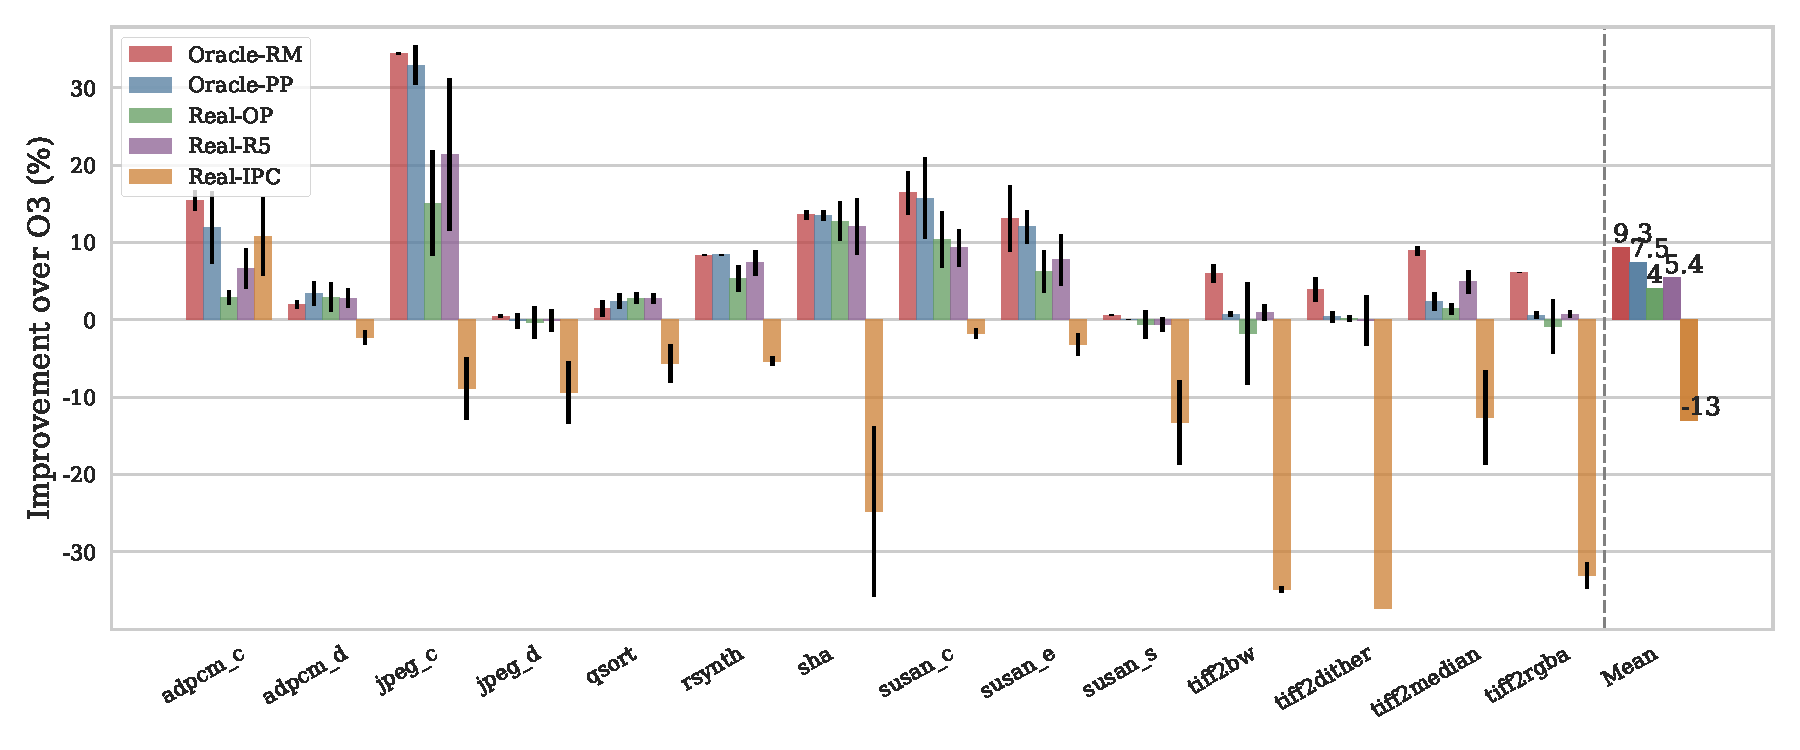
\includegraphics[width=\textwidth]{figs/speedups.pdf}
    \caption{Speedups observed with the online {\itercomp}.}
    \label{fig:speedups}
\end{figure*}

%\begin{figure*}[htb]
%    \centering
%    \includegraphics[width=\textwidth]{figs/profiled-speedups.pdf}
%    \caption{Speedups observed with the online {\itercomp} if we
%             consider the instrumentation overhead.}
%    \label{fig:profiled-speedups}
%\end{figure*}

\subsubsection{Contribution of individual optimisation passes}

Figure~\ref{fig:flagsfreq} shows an aggregated view of the final combination of compiler optimisations that were selected by {\itercomp} search.
The figure presents the individual optimisation passes with at least 1\% of frequency in the selected combination of compiler optimisations that improved the performance over {\texttt{-O3}}.

\begin{figure*}[htb]
    \centering
    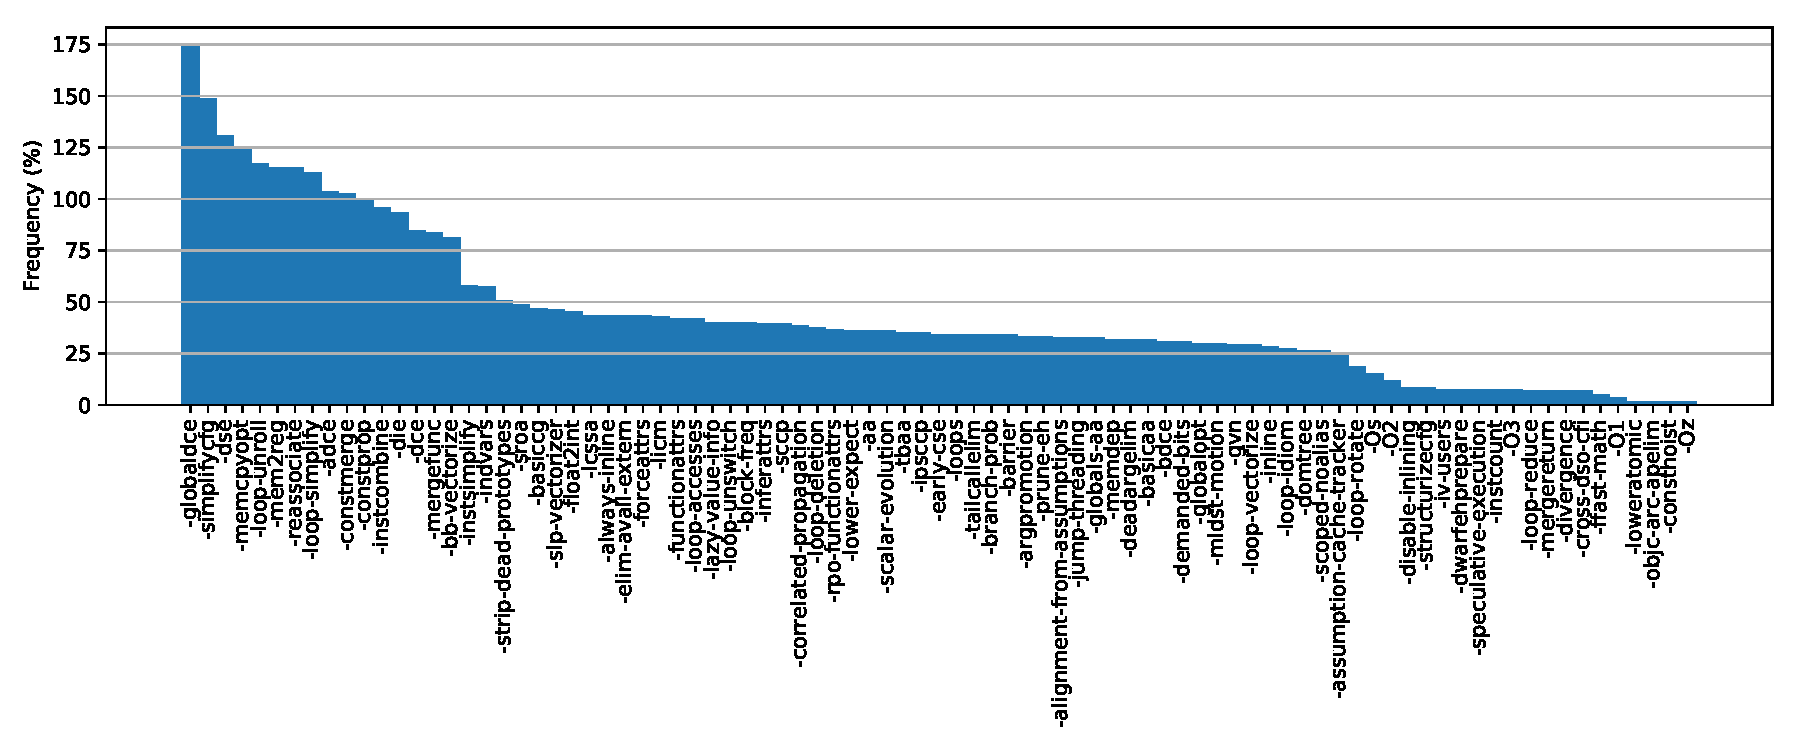
\includegraphics[width=\textwidth]{figs/flagsfreq.pdf}
    \caption{Frequency of individual optimisation passes on the final selected 
             compiler optimisations of the {\itercomp} search over
             all benchmarks.}
    \label{fig:flagsfreq}
\end{figure*}

\section{Summary}

